\section{طراحی دروازه رابط برنامه‌نویسی کاربردی در \lr{Uber}} 
طراحی مناسب دروازه‌های برنامه‌نویسی کاربردی\LTRfootnote{API Gateway} نقش پررنگی در معماری میکروسرویس کاملا دردسترس، قابل توسعه و پیکربندی هم‌زمان با مشاهده‌پذیری بالا دارد. از سال ۲۰۱۴ که \lr{Uber} با رشد چشم‌گیری رو به رو شد و همچنین چندین محصول دیگر نظیر \lr{Uber eat} را نیز بعدا ها ارائه کرد دروازه برنامه‌نویسی کاربردی معماری این شرکت تا کنون چندین نسل تغییرات را تجربه کرده است. \cite{APIGateway}

در ابتدای سال ۲۰۱۴ \lr{Uber} نیز همانند بسیاری از شرکت‌ها با اندازه کوچک و متوسط از یک سرویس اعزام\LTRfootnote{Dispatch service} ساده استفاده می‌کرد و معماری اوبر متشکل از دو سرویس اساسی اعزام و رابط‌کاربردی برنامه‌نویسی \LTRfootnote{API service} بود.سرویس اعزام مسئولیت ارتباط مسافران و رانندگان را بر عهده داشت و سرویس رابط‌کاربردی برنامه‌نویسی مجموعه ای از درخواست‌های خاص را پاسخ می‌داد.


\begin{figure}[h]
\label{fig:apigateway_gen1}
\centering
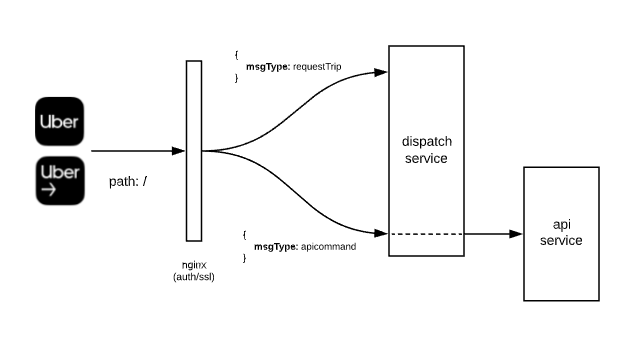
\includegraphics[width=10cm]{gen1_apigateway.png}
\end{figure}

هم برنامه راننده و هم برنامه مسافر با استفاده از یک نقطه انتهایی واحد میزبانی شده در ‘/’ به سرویس اعزام متصل می شوند. بدنه نقطه پایانی دارای یک قسمت خاص به نام \lr{MessageType} بود که دستور \lr{RPC} را برای فراخوانی یک کنترل کننده خاص تعیین می کرد.پیام ها با "\lr{MessageType"} برابر با \lr{ApiCommand} به سرویس رابط‌کاربردی برنامه‌نویسی هدایت می‌شوند.

به فاصله کمتر از یک سال \lr{Uber} با رشد زیاد خود اولین دروازه رابط کاربردی برنامه‌نویسی به معنی واقعی کلمه با قابلیت پاسخ‌گویی به هزاران درخواست در لحظه را هم‌زمان با فراهم‌آوری امکان جستجو مقصد برای کاربران را رونمایی کرد.

دروازه جدید \lr{RTAPI} نامیده شد که اختصار \lr{ Real Time-API} است.در ابتدای سال ۲۰۱۵ دروازه تنها به یک \lr{Restfull API} خدمت می‌داد اما به تدریج تبدیل به یک \lr{Public API} بزرگ شد که به بیش از ۲۰ بستر\LTRfootnote{Platform} متفاوت خدمت می‌کرد.این سرویس یک دروازه واحد بود که با ادامه رشد نمایی به چندین گروه استقرار تخصصی تقسیم شد.
\begin{figure}[h]
\label{fig:apigateway_gen2}
\centering
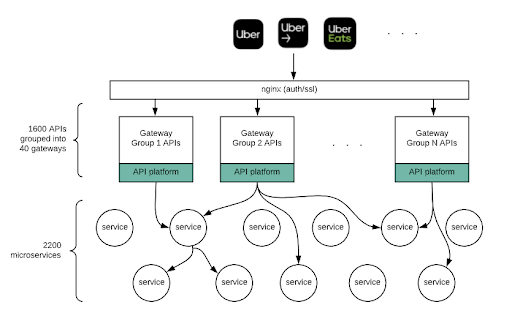
\includegraphics[width=10cm]{gen2_apigateway.png}
\end{figure}

این دروازه با برخی از آمار چشمگیر یکی از بزرگترین برنامه های \lr{NodeJS} در \lr{Uber} بود:
\begin{itemize}
\item
بسیاری از نقاط انتهایی\LTRfootnote{End Point} در 110 گروه‌بندی منطقی نقطه پایانی
\item
پاسخ‌گویی به بیش از ۸۰۰ هزار درخواست در ثانیه
\item
1.2 میلیون ترجمه برای بومی سازی داده ها برای مشتریان انجام شده است
\item
50،000 تست ادغام در هر تفاوت زیر 5 دقیقه اجرا می شود
\item
برای طولانی ترین زمان تقریباً هر روز استقرار وجود داشت
\item
نزدیک به یک میلیون خط کد جریان‌های کاربران را کنترل می‌کردند.
\end{itemize}

100 تیم به طور موازی امکانات جدید را ایجاد می کردند.روزانه تعداد زیادی خدمات جدید از سمت \lr{Backend} ارائه می‌شد و تیم‌های موبایل با همان سرعت در حال ساخت تجربه‌های جدید در محصول بودند. دروازه وابستگی حداقلی میان مولفه‌ها را فراهم کرده و به برنامه های در \lr{Uber} اجازه می‌داد تا به دروازه \lr{API} پایدار و قراردادهایی که ارائه داده است، اعتماد کنند.

اما دروازه به تدریج بزرگ شد و شامل بیش از ۴۰ میکروسرویس مستقل شد که بیش از ۲۵۰۰ بسته \lr{NodeJs} را نیاز داشت و به همین دلیل به روز نگه داشتن بسته‌های مورد استفاده در دروازه با دشواری های بسیاری همراه شد.این بدان معنی است که \lr{Uber} نمی‌توانست آخرین نسخه از کتابخانه های متعدد را استفاده کند. در آن زمان \lr{Uber} شروع به پذیرفتن \lr{gRPC} به عنوان پروتکل جدید خود کرد اما نسخه   \lr{Node.js} در در حال استفاده این امکان را فراهم نمی‌ساخت.

تکرار زیاد موارد استثناهای اشاره‌گر پوچ\LTRfootnote{null pointer exceptions}  که ممکن نبود از آنها در هنگام بازبینی کد و ترافیک سایه\LTRfootnote{Shadow traffic} جلوگیری کرد منجر به متوقف شدن استقرار دروازه رابط کاربردی برنامه‌نویسی برای چند روز شد تا استثنا ها اصلاح شوند و این امر سرعت مهندسی تیم \lr{Uber} را بیشتر کاهش می داد.

در نهایت وجود چنین مشکلاتی سبب شد تا \lr{Uber} به دروازه رابط کاربردی کنونی حرکت کند.
\begin{figure}[h]
\label{fig:apigateway_gen3}
\centering
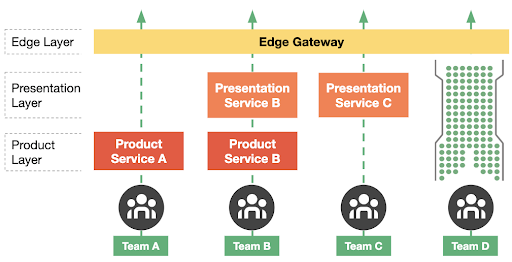
\includegraphics[width=10cm]{gen3_apigateway.png}
\end{figure}
در نهایت مشکلاتی که در نسل دوم دروازه رابط کاربردی برنامه‌نویسی وجود داشت معماران را به ساخت نسل جدید معماری لایه‌ای دروازه تشویق کرد که به صورت مختصر به توضیح آن پرداخت می‌شود.

معماری دروازه معرفی شده شامل بخش های زیر است:
\begin{itemize}
\item
لایه‌ی لبه\LTRfootnote{Edge Layer}: لایه‌ی لبه امکانات زیر را به صورت کامل در اختیار قرار می‌دهد.
\begin{itemize}
\item
Decoupling :
تیم‌های مستقل می‌توانند با حداقل وابستگی به یک دیگر به تولید امکانات بپردازند.
\item
Protocol transformations :
همه ارتباطات بین تلفن همراه به سرور در درجه اول در \lr{HTTP / JSON} است اما از نظر داخلی، \lr{Uber} پروتکل داخلی جدیدی را نیز ارائه کرده است که برای تهیه پروتکل حمل و نقل دو طرفه چند منظوره ساخته شده است و همین موضوع تبدیل این پروتکل‌ها به \lr{HTTP/JSON} را ضروری می‌سازد.
\item
Crosscutting concerns :
تمام رابط های برنامه کاربردی مورد استفاده شرکت مورد نیاز یک سری عملکرد خاص است که باید معمول و قوی باقی بماند.
\item
Streaming payloads:
ارسال \lr{Push notification} به موبایل‌ها باید توسط سیستم واحد مدیریت جریان داده صورت پذیرد.
\end{itemize}
\item
لایه نمایش \LTRfootnote{Presentation Layer}:
میکروسرویس‌ها که به طور خاص برای دست‌یابی به یک هدف پیاده‌سازی شده اند تا ویژگی ها و محصولات خود را برای قسمت \lr{FrontEnd} ارائه دهند. این روش منجر به این می شود که تیم های تولیدی خدمات ارائه و ارکستراسیون خود را که \lr{API} مورد نیاز برنامه های مصرف کننده را برآورده می کنند، مدیریت کنند.
\item
لایه محصول\lr{Product Layer}:
لایه محصول به پیاده‌سازی امکانات برای محصولات خاص اختصاص داده شده است.
\item
لایه دامنه\lr{Domain Layer}:
شامل میکروسرویسها که گره برگ که قابلیت خاص منظوره شده‌ای را تنها برای یک تیم محصول فراهم می کند.
\end{itemize}